{
\setlength{\parindent}{2em}
\section{Black Box Symbol Access}\label{sec:das-mem-restore}
It was mentioned previously that, for integration reasons, the flight software code was considered unalterable (through requirement U02). Modifying the \gls{FSW} to accommodate the new checkpointing feature in BBPSim clearly defeated the purpose of encapsulation, and could potentially introduce errors in a critical piece of software. To represent reality as much as possible, the FSW was supposed to contain as fewer indications of the existence of \gls{BBPSim} as possible in its code.

In \autoref{sec:conditions}, it was shown that saving the entire set of statically-allocated variables in the DAS domain was a necessary condition for a stable restore. However, as it was forbidden to add \textit{getter} functions (e.g. \mintinline{c}|GetTheVariable()|) to access file-local variables from BBPSim, there needed to be a different solution. For the save and restore to be properly integrated, there needed to be a way to access them at runtime, a kind of indirect or "black box" access. 

In the end, the solution that was adopted involved the handling of DAS object files, \textit{after} they were compiled. Ultimately, no control over the flight software source code was given, but the compilation and building process were alterable. The following sections show how this limited control could be harvested, using a series of manipulations at build time, to give the \gls{BBPSim}-domain objects the required access to save the state of the flight software.

\subsection*{Linking Process}
First of all, it is crucial to understand how the linking process of an application is done. As mentioned earlier, when each source code file is compiled by \gls{GCC}, a \texttt{.o} object file is produced. Although this file contains executable code, the object file that would be produced by GCC would, by itself, not be enough to be executable as a stand-alone. The \textit{linker} needs to first process the object files. The one used in the case of this thesis was GNU \texttt{ld} version 2.27.

\begin{figure}[htbp]
	\centering 
	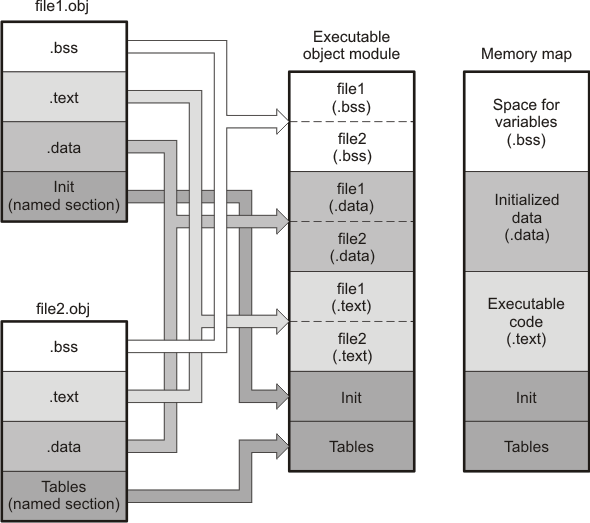
\includegraphics[width=.75\linewidth,keepaspectratio]{art/obj-to-elf-to-mem.png}
	\caption{Combining Input Sections to Form an Executable Object Module.\cite{online:linking}}
	\label{fig:link-mult-files}
\end{figure}

The linker's role in the building process is to combine each of the object files given as input into an executable file, or in the case of this thesis, a dynamic library. \autoref{fig:link-mult-files} better illustrates that concept. At linking time, \texttt{ld} groups the same segments from each \texttt{.o} file together and lays them sequentially in the executable object. Since object files can be given in an arbitrary order, the linker can make no guarantee on the final layout on its own.

In addition, while combining the object files together, the linker also resolves the undefined \textit{external} symbols, variables declared in one object file but used in another. 

Just like source code determines the resulting output of the compiler, it is also possible to control the linking process through the use of a linker script\cite{online:ld-scripts}. Even though, in most cases, users of the GNU linker don't provide a custom script, it is possible to specify one at linking time. 

Using such a script offers much more granularity to the developer in terms of which section gets put where in the executable object. In the field of embedded systems, this is particularly useful. Since components like non-volatile flash memory can be adressable by the CPU\cite{online:flash-ram}, it lets the developer decide whether certain sections should be written to flash (e.g. addressed from 0x10000 to 0x50000) or just be allocated in RAM before running the program.

\begin{listing}[H]
	\vspace{12pt}
	\begin{minted}{c}
SECTIONS
{
	. = 0x10000;
	.text : { *(.text) }//$\label{line:link-ex}$
	. = 0x8000000;
	.data : { *(.data) }
	.bss : { *(.bss) }
}
	\end{minted}
	\caption{Simple example of a GNU \texttt{ld} linker script.}
	\label{code:link-script-ex}
\end{listing}

One can read the example linker script in \autoref{code:link-script-ex}  sequentially. On line \ref{line:link-ex}, the script lays out the \texttt{.text} sections of all the object files sequentially inside the executable object's own \texttt{.text} section. This newly created section starts at address 0x10000 (represented by the "." keyword, the \textit{location counter}\cite{online:gnu-ld}). Then, the linker does the same thing for the \texttt{.data} and \texttt{.bss} sections, starting at address 0x8000000.

\subsection*{Clustering Flight Software Sections}
Since managing memory is always easier when it is contiguous, the first step that was taken to access the flight software memory was to group the sections of the relevant files together. This was done using a custom linker script. To make sure not to leave out any section, the default GNU \texttt{ld} linker script was used to make sure to start from a valid point. This script could be outputted from a shell with 
\begin{minted}{bash}
ld --verbose
\end{minted}
From that point, it was possible to partition the essential sections of the DAS object files only by changing the already valid script. These sections could be clustered in a special section of an intermediate shared object \pathmono{libBbpSim-intermediate.so}. 

As previously stated, one of the linker's job when building an executable is to resolve undefined symbols across all object files and to "interlink" them together. To do that, \texttt{ld} starts by looking in other object files to locate and set the correct addresses. Despite that, if said symbols are not defined in any object files, \textit{they can also be defined in the linker script}. This has two major implications: 
\begin{enumerate}
	\item Bi-directional transmission of values is possible (C code $\Longleftrightarrow$ linker).
	\item The source code can never know in advance the value of the undefined symbol if it's only defined during the linking phase.
\end{enumerate}

By harvesting these concepts together, two new contiguous sections of DAS variables in \pathmono{libBbpSim-intermediate.so} could be constructed. They are shown in \autoref{code:link-script-das}. For both the new \texttt{.das_state_vars_bss} and \texttt{.das_state_vars_data} sections, two symbols were defined as boundary variables to identify the start and end of the section in memory. A pair can be seen at lines \ref{line:bound-start} and \ref{line:bound-end}.

\begin{listing}[htbp]
	\vspace{12pt}
	\begin{minted}{c}
//...
.das_state_vars_data :
{
	__das_state_vars_data_start = .;//$\label{line:bound-start}$
	SORT(*obj/DasSrc/ *.o)(.data .data.* .gnu.linkonce.d.*)
	__das_state_vars_data_end = .;//$\label{line:bound-end}$
}
.das_state_vars_bss (NOLOAD) :
{
	__das_state_vars_bss_start = .;
	SORT(*obj/DasSrc/ *.o)(.bss .bss.* COMMON)
	__das_state_vars_bss_end = .;
}
//...
	\end{minted}
	\caption{Clustering of DAS variables via the \texttt{ld} linker script.}
	\label{code:link-script-das}
\end{listing}

It should also be noted that the \texttt{NOLOAD} parameter of the new \texttt{.das_state_vars_bss} section informed the linker that this memory section was to be zeroed out when the library was loaded, and thus not to allocate this memory inside the shared object itself. Otherwise, the library would be composed of nearly 100MB of zeros. And thanks to the inclusion of section guards, it was now possible to access the start and end addresses of the sections from C using:
\begin{minted}{c}
extern char __das_state_vars_data_start[];
extern char __das_state_vars_data_end[];
\end{minted}

To confirm that the script worked, an output map was produced by \texttt{ld} after the linking process (using \texttt{-Wl,-M=mapfile.map}). An excerpt is given in \autoref{map:ld}. It shows that the sections get created and that the \texttt{.data} and \texttt{.bss} sections of each DAS object file all get correctly mapped in the output file.

\subsection*{Cataloging State Variables}
Once the relevant sections of memory related to DAS were correctly laid out after the linking process, it was now a matter of deducing the address of each of these variables inside the resulting shared object. As the outputted file was in the ELF format, an ELF analyzing program could then be used to get the list of all the variables contained within the relevant section:
\begin{minted}{bash}
objdump --syms -j .das_state_vars_data libBbpSim-intermediate.so
\end{minted}
Once the output was sanitized with \texttt{awk}, a big text file represented in  \autoref{das-symbol-catalog} was produced. This was called the \textit{symbol catalog}. One can observe various components in this file:
\begin{enumerate}
	\item The first line contains the SHA1 sum of the entire DAS source code repository. This was added to associate the list of variables to an existing source code for compatibility purposes.
	\item Each additional line represents a symbol that is contained in the flight software domain. They are laid out in the \verb|[<address> <size> <name>]| format. The addresses and the sizes are outputted in hexadecimal.
	\item The symbols defined as "guards" (\texttt{__das_state_vars_data_start}) earlier in the linker script were also included in this list. Because they don't represent any value in source code but instead hold an address, their size was zero.
\end{enumerate}

\subsection*{Including the Catalog in the Library}
Being able to generate a symbol catalog was very useful. However, there was a problem: with the way it was constructed, that catalog could never be included in the library. The catalog was generated from a finished shared object, but for it to ever be useful, the catalog needed to be accessible by the library at runtime. This created a chicken and egg problem, where both artifacts were dependent on one another.

The dependence was bypassed by transforming the symbol catalog into an object file and re-linking the library once again, including the new transformed catalog. 

Embedding raw bytes inside an executable file has been done since the early days of computing. For instance, it is possible for a malicious programmer to embed executable code within a self-extracting archive file\cite{online:sfx}. In the case of BBPSim, which was an ELF running on an x86 64-bit machine, it was possible to embed the catalog, as a string, \textit{inside} the library itself by first transforming it into a \texttt{.o} file:
\begin{minted}{bash}
objcopy --input binary --output elf64-x86-64          \
--binary-architecture i386:x86-64                     \
--rename-section .data=.das_state_vars_catalog_string \
das-symbol-catalog.txt                                
\end{minted}

This put the raw bytes of the catalog in the \texttt{.das_state_vars_catalog_string} section of the \pathmono{das-symbol-catalog.o} file.

The second part consisted in correctly laying out those bytes in the second and final shared object, \pathmono{libBbpSim.so}. This was done by once again taking advantage of the linker script in \autoref{code:link-script-das} to add an additional section, \texttt{.das_state_vars_catalog_string}.

Finally, all the object files both from the BBPSim and DAS domains could be linked a second time, together with \pathmono{das-symbol-catalog.o}. The resulting \pathmono{libBbpSim.so} file would be the last and final shared object. This effectively embedded the symbol catalog's raw bytes, encoded in \gls{ASCII} characters. Executable code inside the library could also refer to the stringized symbol catalog using newly created symbols used as guards for the raw bytes. Those symbols being only defined in the second linking process, it was necessary to tag them as having \texttt{weak} linkage for the linker not to complain on the first linker pass:
\begin{minted}{c}
extern char __attribute__((weak)) _binary_das_symbol_catalog_txt_start[];
extern char __attribute__((weak)) _binary_das_symbol_catalog_txt_end[];
\end{minted}

The results can be better shown by using a binary visualization program\cite{online:binvisio}. \autoref{fig:bin-lib-comp} shows a comparison of the \pathmono{libBbpSim-intermediate.so} and \pathmono{libBbpSim.so} shared objects in binary. Bytes with a value in the \gls{ASCII} character range are represented in blue. Both images read left-to-right with address 0x0 on the left. It is possible to see that a new blue section appears in \autoref{fig:bin-lib-final}, thus confirming that the symbol catalog correctly gets included in the final version of the BBPSim library.

\begin{figure}[htbp]
	\centering
	\begin{subfigure}{\linewidth}
		\centering
		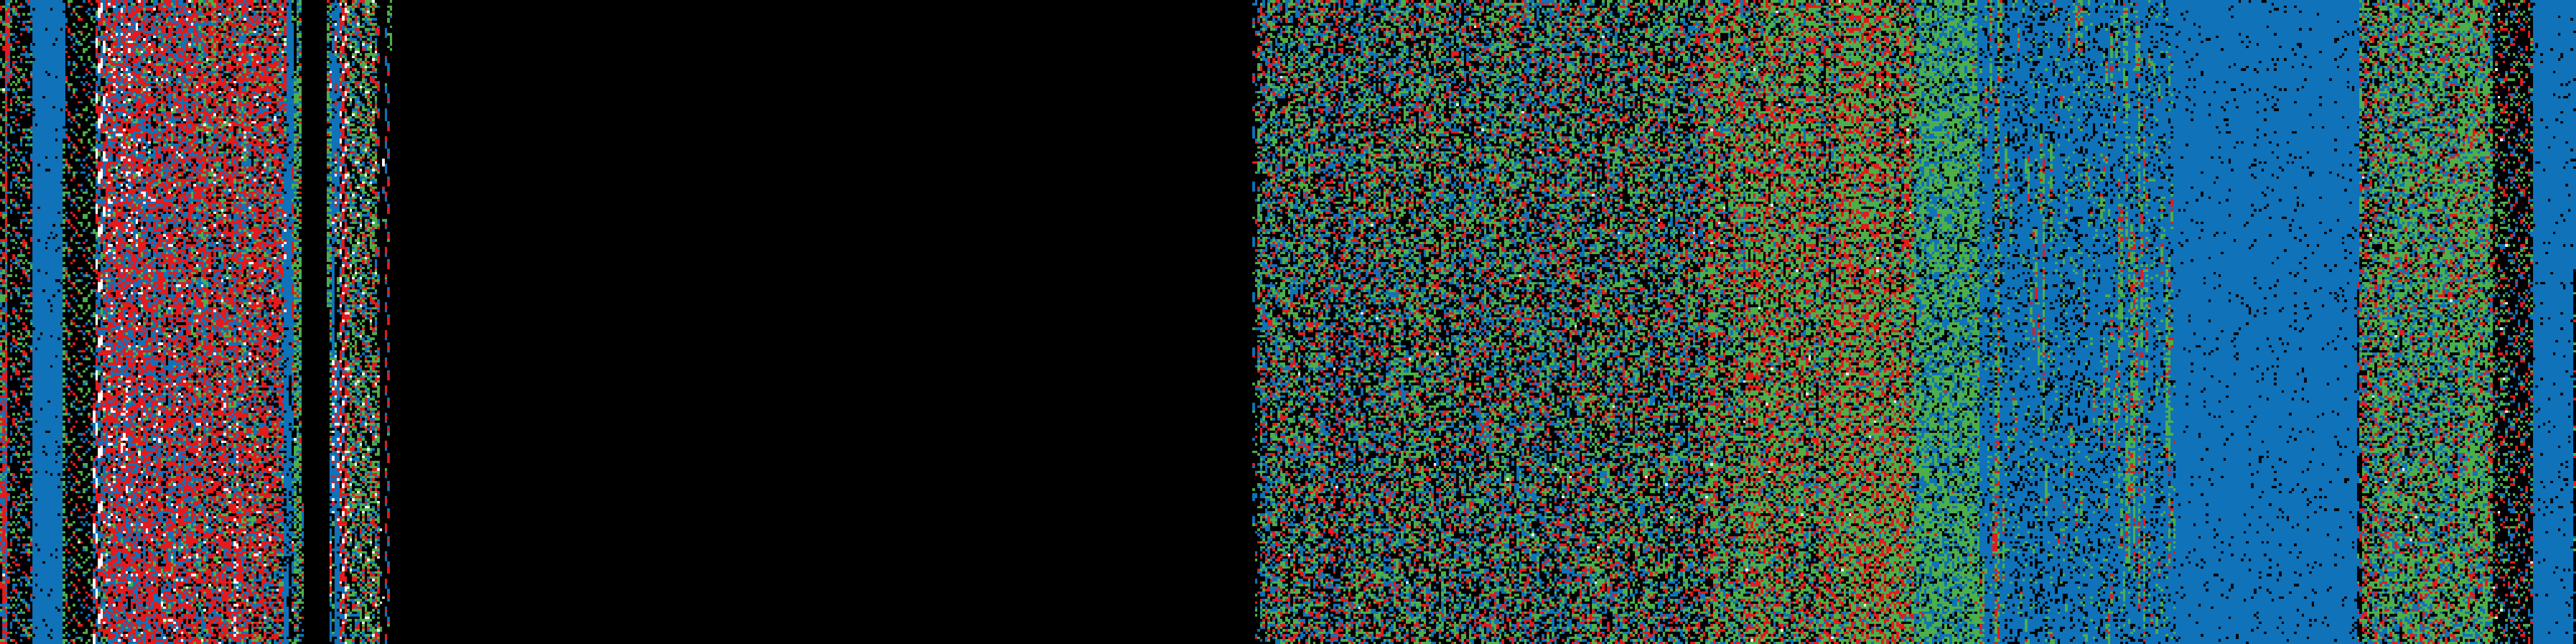
\includegraphics[width=\linewidth, keepaspectratio]{art/bin-lib-intermediate.png}
		\caption{Binary visualization of \pathmono{libBbpSim-intermediate.so}}
		\label{fig:bin-lib-intermediate}
	\end{subfigure}
	\vspace{12pt}
	\begin{subfigure}{\linewidth}
		\centering
		\includegraphics[width=\linewidth]{art/bin-lib-final.png}
		\caption{Binary visualization of \pathmono{libBbpSim.so}}
		\label{fig:bin-lib-final}
	\end{subfigure}
	\caption{Comparison of the resulting libraries after the first and second linking process.}
	\label{fig:bin-lib-comp}
\end{figure}

Since there is no modification to the DAS object files between the two linking process, the variable list taken from \pathmono{libBbpSim-intermediate.so} \textit{is guaranteed} to be the same and in the same order as \pathmono{libBbpSim.so}. 

\subsection*{Shared Object Considerations}
- Dynamic library loading  https://eli.thegreenplace.net/2011/08/25/load-time-relocation-of-shared-libraries
- address at which the library is loaded (why alwayshttps://unix.stackexchange.com/questions/509607/how-a-64-bit-process-virtual-address-space-is-divided-in-linux 0x00007fffXXXXXXXX?) 
In this case, application continerization is not possible, because we are a library.
- how to access everything (talk about dynamic library loading, elf dumps, double linking etc.)

\subsection*{Summary}
The whole process from is quite complex. With this manipulation of sections, one can get easily confused. This is why the whole process is 
}